\section{Common use cases for replicated state machines}
\label{motivation:uses}

Replicated state machines are a general-purpose building block for making
systems fault-tolerant. They can be used in a variety of ways, and this
section discusses some typical usage patterns.

\begin{figure}
\hfill
\begin{subfigure}{.45\textwidth}
\centering
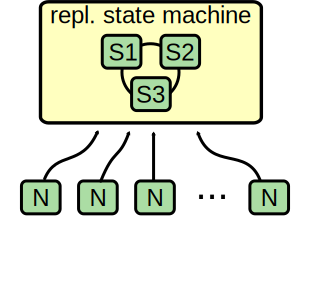
\includegraphics[scale=.5]{motivation/activeactive}
\caption{
The nodes in the cluster coordinate among themselves by reading from and
writing to the replicated state machine.
\\
}
\label{fig:motivation:activeactive}
\end{subfigure}
\hfill
\begin{subfigure}{.45\textwidth}
\centering
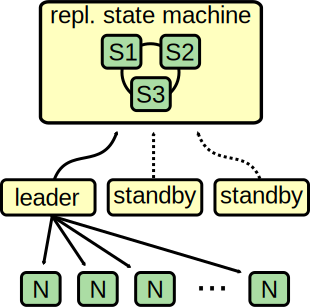
\includegraphics[scale=.5]{motivation/activepassive}
\caption{
One leader actively manages the nodes in the cluster and records its
state using the replicated state machine. Other standby servers are
passive until the leader fails.
}
\label{fig:motivation:activepassive}
\end{subfigure}
\hfill
\vcaption[common patterns for using a single replicated state machine]{
Common patterns for using a single replicated state machine.
}
\end{figure}


Most common deployments of consensus have just three or five servers
forming one replicated state machine. Other servers can then use this
state machine to coordinate their activities, as shown in
Figure~\ref{fig:motivation:activeactive}. These systems often use the
replicated state machine to provide
group membership, configuration management, or locks~\cite{Hunt:2010}.
As a more specific example, the replicated state machine could provide a
fault-tolerant work queue, and other servers could coordinate using the
replicated state machine to assign work to themselves.

A common simplification to this usage is shown in
Figure~\ref{fig:motivation:activepassive}. In this pattern, one
server acts as leader, managing the rest of the servers.
The leader stores its critical data in the consensus system.
In case it fails, other standby servers compete for the position of
leader, and if they succeed, they use the data in the consensus system
to continue operations.
Many large-scale storage systems that have a single cluster leader, such as
GFS~\cite{Ghemawat:2003}, HDFS~\cite{Shvachko:2010}, and
RAMCloud~\cite{Ousterhout:2011}, use this approach.

\begin{figure}
\centering
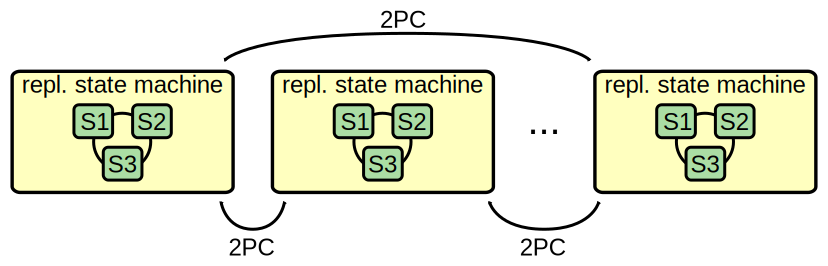
\includegraphics[scale=.5]{motivation/bigdata}
\vcaption[partitioned large-scale storage system using consensus]{
Partitioned large-scale storage system using consensus.
For scale, data is partitioned across many replicated state machines.
Operations that span partitions use a two-phase commit protocol.
}
\label{fig:motivation:bigdata}
\end{figure}

Consensus is also sometimes used to replicate very large amounts of
data, as shown in Figure~\ref{fig:motivation:bigdata}. Large storage
systems, such as Megastore~\cite{Baker:2011},
Spanner~\cite{Corbett:2012}, and Scatter~\cite{Glendenning:2011},
store too much data to fit in a single group
of servers. They partition their data across many replicated state machines,
and operations that span multiple partitions use a two-phase commit
protocol (2PC) to
maintain consistency.


